We test AJFS on a local machine as well as sysnet cluster. The evaluation includes consistency part and performance part.

\subsection{Consistency}

The main design purpose of AJFS is the file consistency when accessed by multiple servers. We've tested the following cases:

\subsubsection{Server crash and rejoin}

In distributed system, it's common that server crashes. We need to guarantee that when a server is down, the data is not corrupted and when the server is back online, the data will be synchronized.

The design of AJFS supports server rejoin. Since it's running based on the local backup, client can access the file locally without issue, just like Coda~\cite{KS92} does.
The only problem is when the server is down, client cannot access the mount point, because fuse server is also down. Instead, client should access the local backup. When the server rejoins, it will automatiaclly rsync with remote repositories and sync up the local files with remote replicas.

We tested following test cases on AJFS:

1. Start three AJFS servers A, B and C; kill server C; client a on server A creates file x; restart server C.

\emph{Result}: client c on Server C can get file x automatically.

The test proves AJFS's robustness: server can join and crash randomly, but file consistency is kept among replicas.

\subsubsection{Write protection}

Many distributed systems support mulitple simultaneous writes. TreadMarks~\cite{treadmarks} supports multiple writers; Bayou~\cite{bayou} askes each writer to provide dependency check and merge procedures.
AJFS does not support multiple simultaneous writers though, this is mainly for simplicity reason. 

A possible solution to support multiple simultaneous writers in AJFS is copy on write. The write operation only writes to the local copy, and when the file is closed, the modifications is propagated to the replicas. We do not use this mechanism because the merge procedure on server the side may be complicated. Another solution to this issue is to keep different conflict versions of a single file. 
However, we choose locks and only allow one writer to a file at one time, which is simple and the correctness is guaranteed.

We tested following test cases on AJFS:

1. Client a on server A writes to file x; at the same time client b on sever B opens file x for read.

2. Client a on server A writes to file x; at the same time client b on sever B opens file x for write.

3. Client a on server A read file x; at the same time client b on sever B deletes the folder which contains file x.

On AJFS, all the test cases work as expected; For test case 1, client b can open the file for read, because we allow one writer and multiple readers simultaneously. For test case 2, the request from client b is declined. For test case 3, AJFS denies the operation, specifies the folder is not empty. Hence we guarantee the file consistency on AJFS.

\subsection{Performance}

Performance is not the key motivation of AJFS. Use AJFS to sync up big files is not efficient, this is because AJFS needs to propagate the data to all the nodes during the write.
However, AJFS supports big file sync up.

Figure \ref{figure:writeperf} shows the performance of AJFS write, which is measured using dd.
There is a clear trend that with the number of AJFS nodes increasing,
the write bandwidth of AJFS decreases. This is because although AJFS uses asynchronous write propagation, that it does not wait for the response from remote nodes,
transfer the data itself adds additional overhead. 
More nodes means more data needs to transfer, hence the performance degrades with the number of nodes increasing.
That's why AJFS does not suit for big files sync up.

We can optimize the write performance by using additional thread, which queues up write requests and propagate them to remote nodes asynchronously.
This will improve the write performance of AJFS and makes the write performance constant.

\ref{figure:readperf} shows the read performance of AJFS. It is constant with number of nodes increasing, and is also close to Fuse read performance.
This is because AJFS handles read locally and does not propagate non-modification request.
%However, we compare the AJFS system with a local filesystem. The test is run by bonnie++ 1.03e~\cite{bonnie++}. Table \ref{table:performance} shows the AJFS bandwidth performance. 

As we can see, since FUSE is a user space file system, it adds additional
 overhead to the file operations and hence the performance is worse than the local file system.
Also, the write performance of AJFS is lower than FUSE with number of nodes increasing, as it needs to propagate the requests to all the remote nodes.
 This is a limitation with current AJFS implementation and can be resolved by propagating write requests asynchronously.

\begin{figure}[Ht]
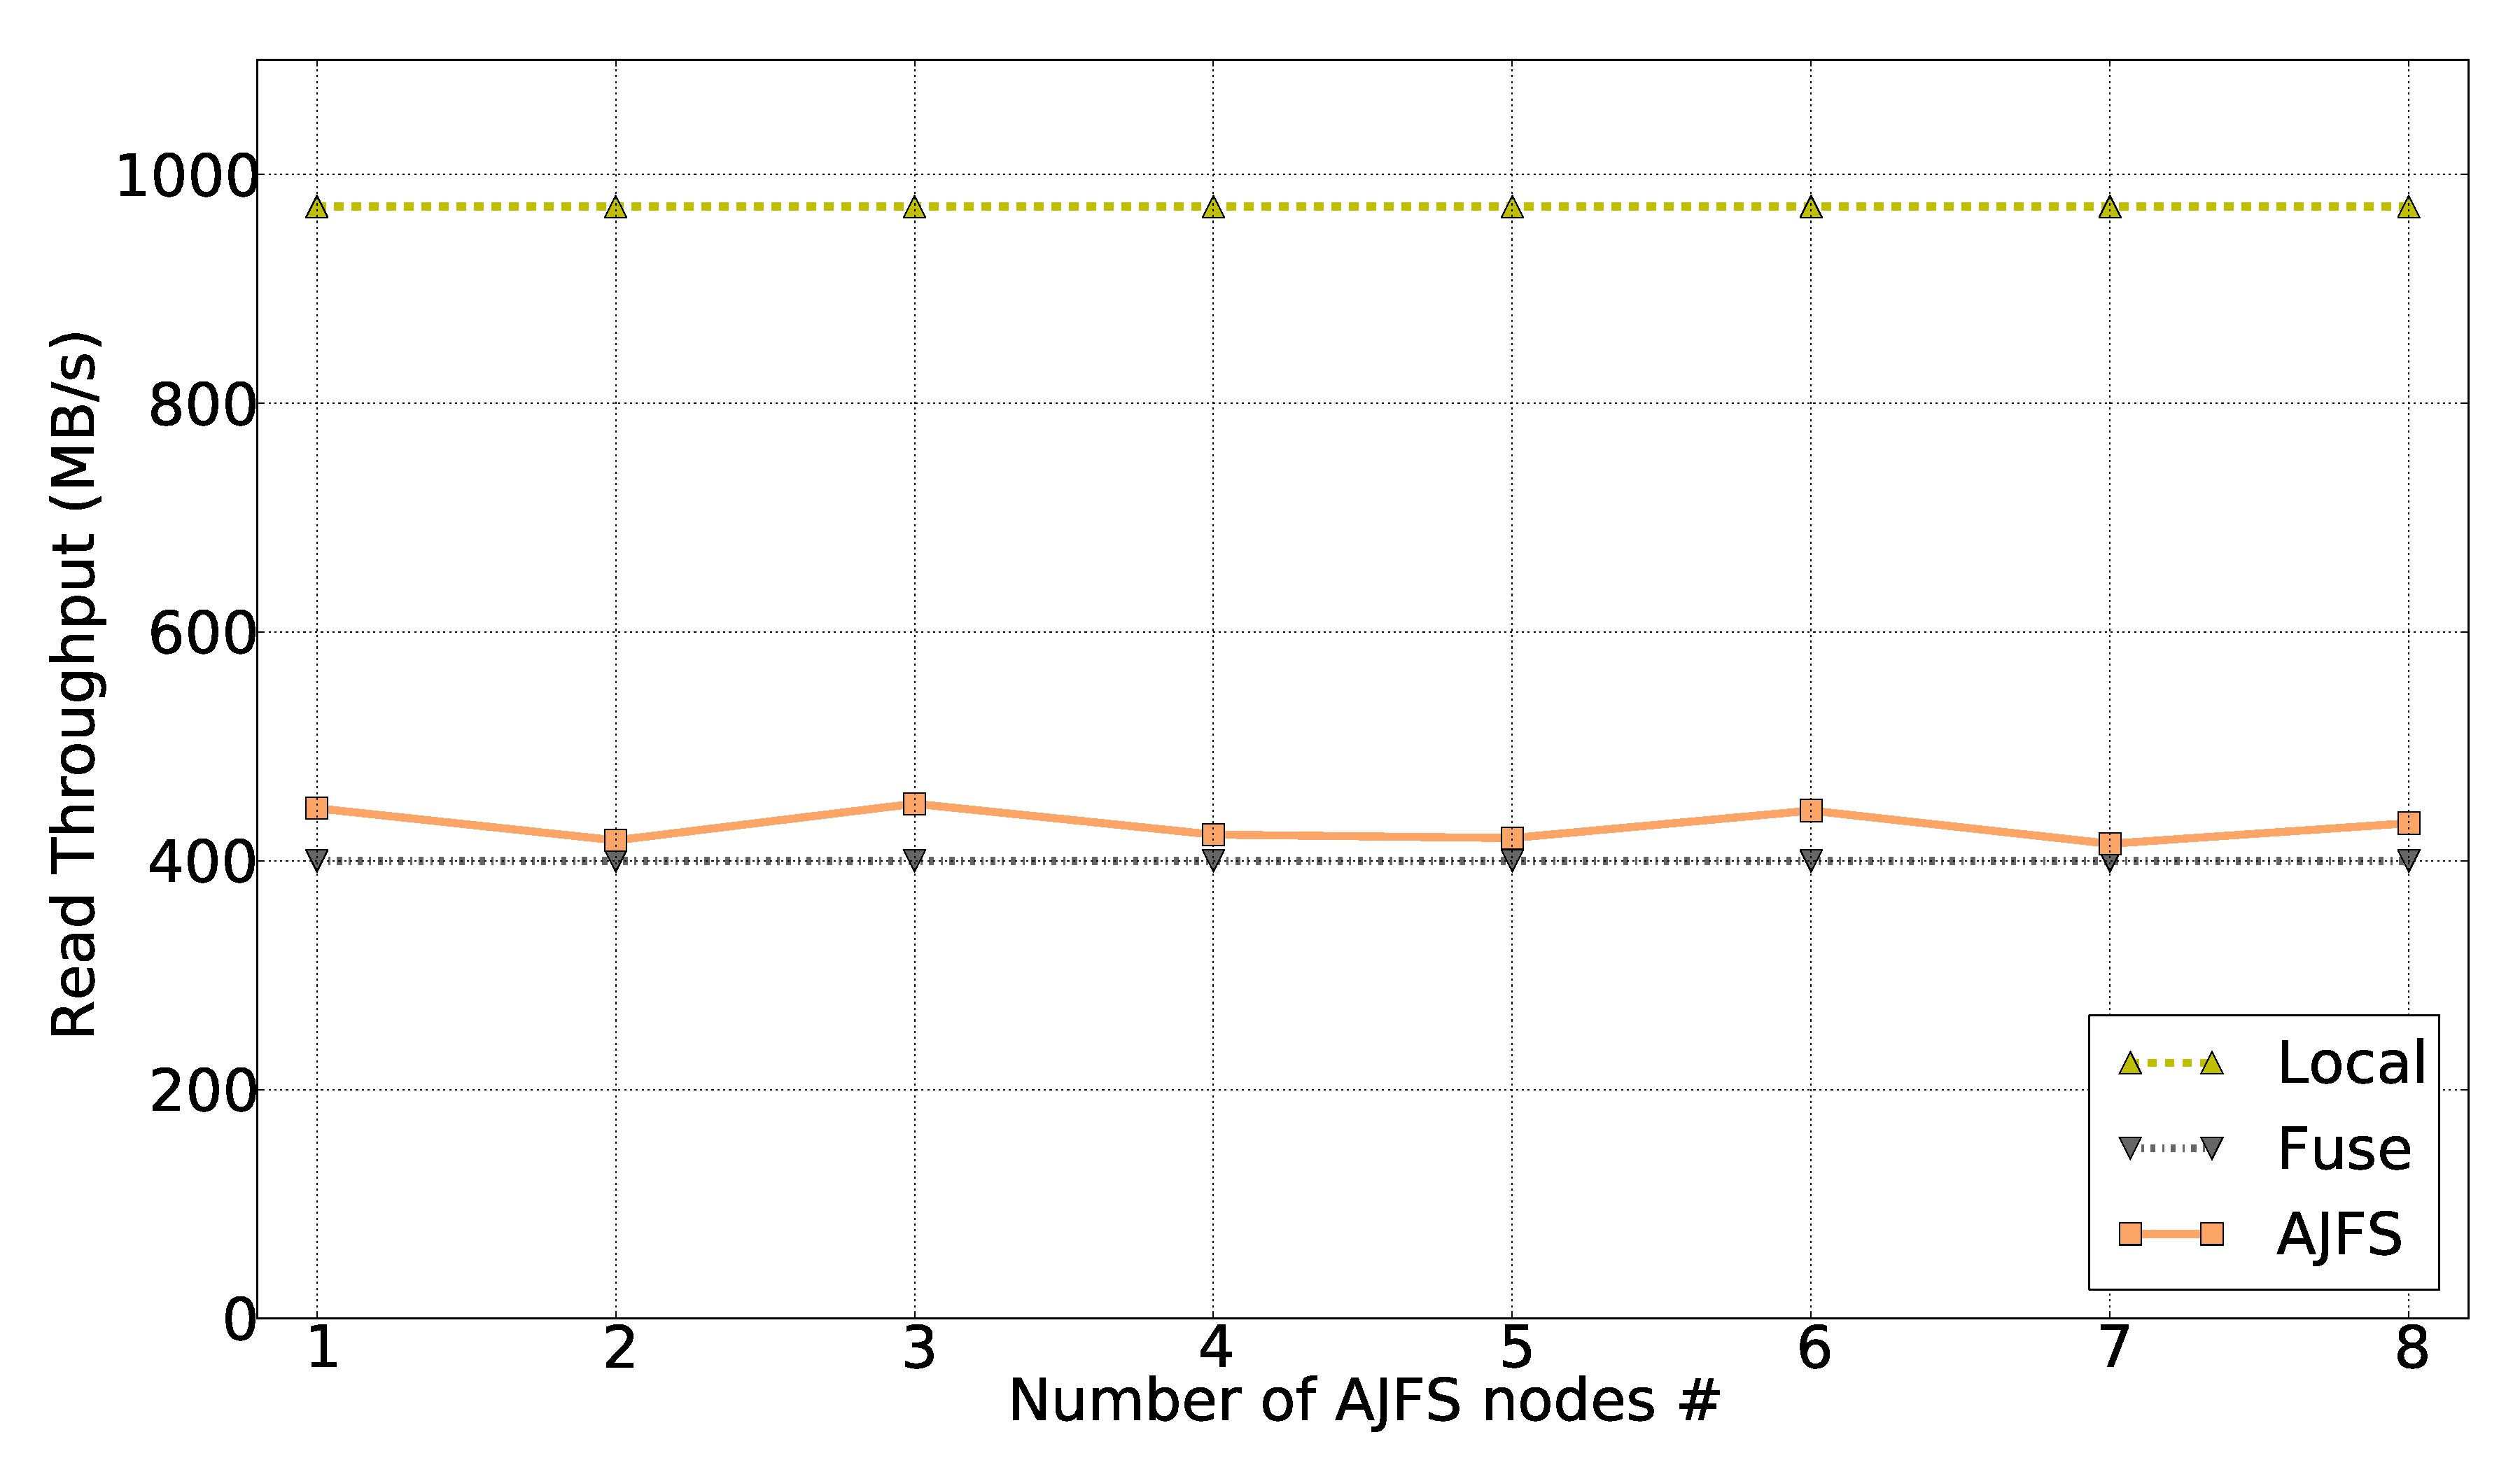
\includegraphics[width=\linewidth]{readperf.pdf}
\caption{AJFS Read Performance}
\label{fig:readperf}
\vspace{-5mm}
\end{figure}

\begin{figure}[Ht]
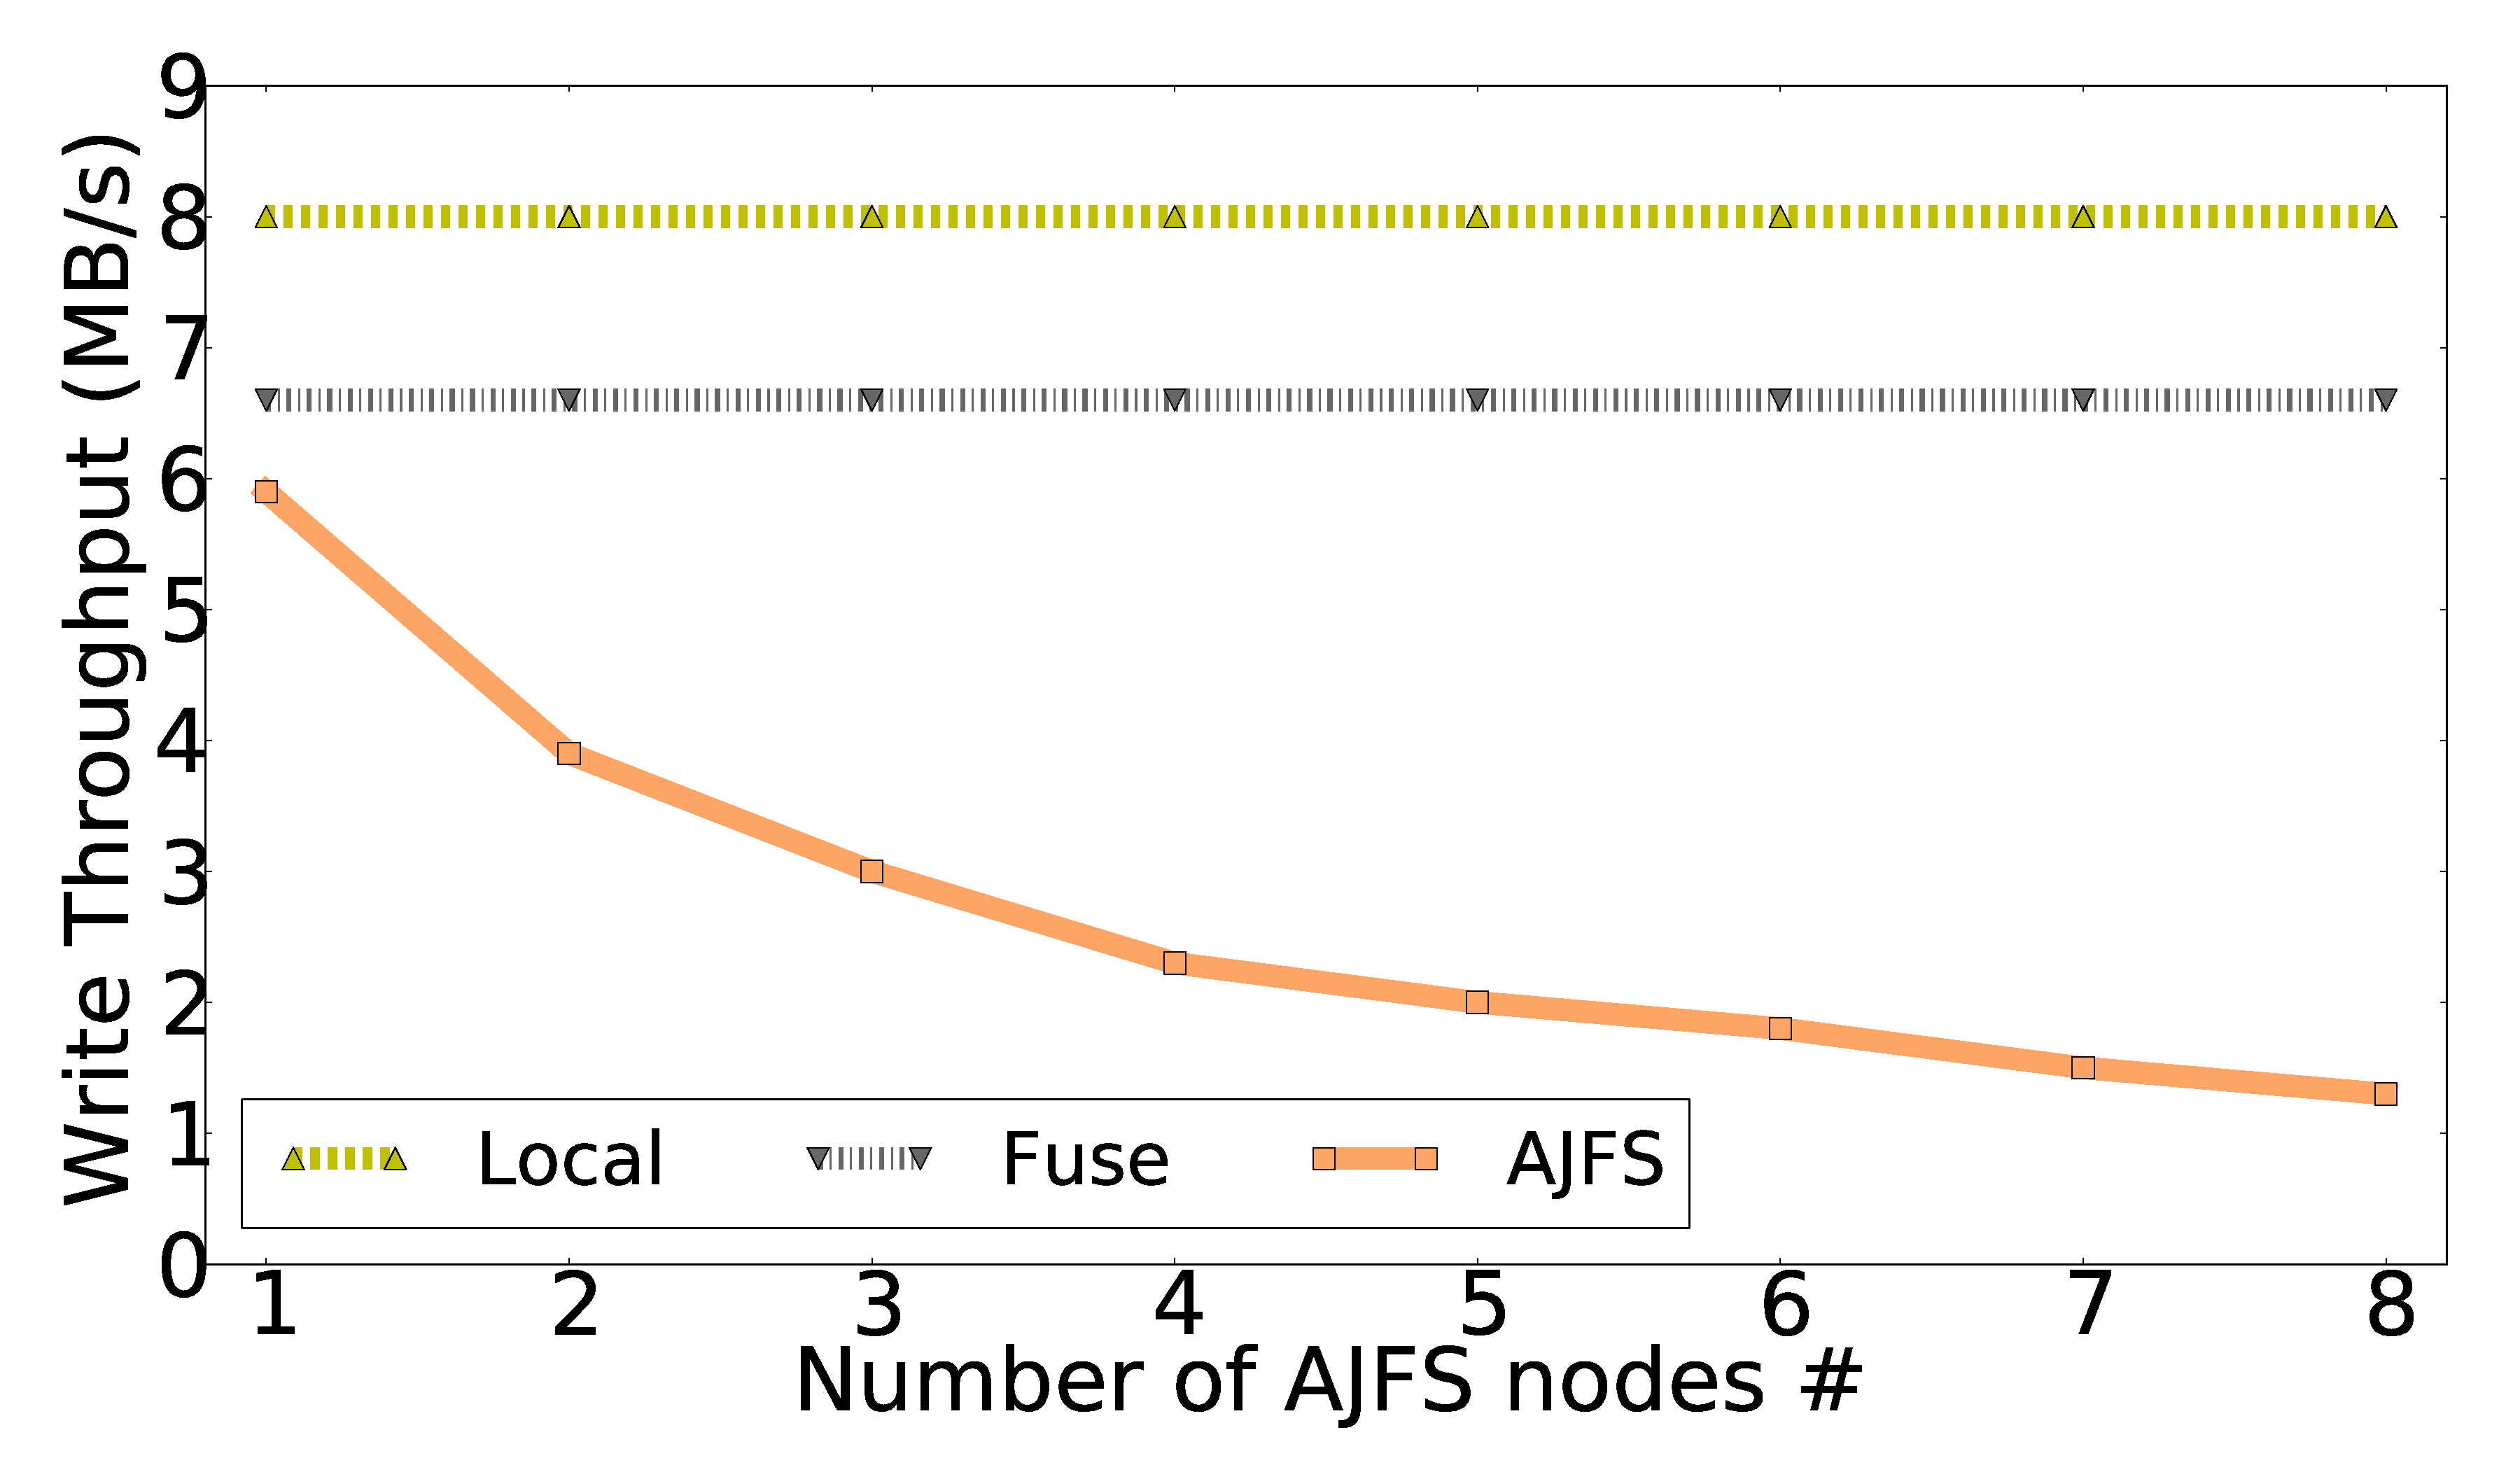
\includegraphics[width=\linewidth]{writeperf.pdf}
\caption{AJFS Write Performance}
\label{fig:writeperf}
\vspace{-5mm}
\end{figure}

\begin{table}[Ht]
\caption{AJFS read/write performance (KB/s)}
\centering
\begin{tabular}{|p{0.9cm}|p{0.9cm}|p{0.9cm}|p{0.9cm}|p{0.9cm}|p{0.9cm}|}
\hline\hline
System & Byte Write & Block Write & Rewrite & Byte Read & Block Read \\
%heading
\hline
Ext3	& 49090	& 55403	& 17766	& 45094	& 66464	\\
\hline
FUSE	& 33792	& 47490	& 15417	& 39853	& 78666	\\
\hline
AJFS	& 13972	& 19651	& 11383	& 41987	& 74125	\\
\hline
\end{tabular}
\label{table:performance}
\end{table}
